%Phone 
%open chapters on any page, final removes formatting marks
\documentclass[10pt,openany,final]{memoir}
\title{Thoughts About IF}
%place graphics package first to avoid conflicts (weird page sizes)
\usepackage{graphicx}
\usepackage{wrapfig}


%\usepackage[paperwidth=70.9mm, paperheight=143.6mm, hmargin={1cm, 1cm},vmargin={1.2cm, 1.25cm}]{geometry}
% New setup
% setstocksize{height}{width}
\setstocksize{216mm}{137mm}
\settrimmedsize{216mm}{137mm}{*}
\settypeblocksize{216mm}{137mm}{*}
\setlrmarginsandblock{24.0mm}{24.0mm}{*}
\setulmarginsandblock{27mm}{27mm}{*}
% \marginparmargin{2mm}
% memoir: finalize the page changes
\checkandfixthelayout

\usepackage{microtype}

% \usepackage{marginnote}
%\usepackage{wrapfig}
%\setbeforesecskip{2mm}
% \setaftersecskip{2mm}
%\setSindent{0pt}

% TYPEFACE PROPERTIES
%--------------------
% fontspec system for typeface definitions
\usepackage{fontspec,xunicode,polyglossia}

%NOTE: good discussion of fonts: https://tex.stackexchange.com/questions/352804/setmainfont-vs-fontspec
%letter spacing

%fontspec font selection
\setmainfont{LinuxLibertineG}[
BoldFont = LinuxLibertineGB,
ItalicFont = LinuxLibertineGI,
BoldItalicFont = LinuxLibertineGZI,
SlantedFont = LinLibertineSlantedZ,
BoldSlantedFont = LinLibertineSlantedZ,
SmallCapsFont = LinLibertineCapitals
]
\setmonofont{LinLibertine_M}
\setsansfont{LiberationSans}


\makeatletter
%\g@addto@macro\chapnamefont{\sffamily} 
%\g@addto@macro\chapnumfont{\sffamily}  
%\g@addto@macro\chaptitlefont{\sffamily}
%\makeatother

% PAGE PROPERTIES
%----------------
%% common ligatures
%TODO: add more ligatures
\usepackage{newunicodechar}
\newunicodechar{ff}{ff}
\newunicodechar{fi}{fi}
\newunicodechar{fl}{fl}
\newunicodechar{ffi}{ffi}
\newunicodechar{ffl}{ffl}
%% end of common ligatures

% CHAPTER PROPERTIES
%-------------------

% remove chapter number from the page headers
% \addtopsmarks{headings}{}{
%   \createmark{chapter}{left}{nonumber}{}{}
% }
% \pagestyle{headings} % activate changes


%chapter page style
\makechapterstyle{plroman}{
\renewcommand\printchaptername{}
\renewcommand\printchapternum{\centering\MakeUppercase
{\fontsize{.75in}{1in}\selectfont\romannumeral\thechapter}}
\renewcommand\afterchaptertitle{\vskip0.25\midchapskip\vskip\midchapskip
\hrule\vskip0.15\midchapskip\vskip\midchapskip}
}

% Use this chapter style
\chapterstyle{plroman}

% Drop first letter of each chapter
\usepackage{lettrine}

% Precise colors
\usepackage[dvipsnames,svgnames,table]{xcolor}

%flexible margin notes
\usepackage{marginnote}

% PAGE HEADER PROPERTIES
% -----------------------
\nouppercaseheads
\makepagestyle{mystyle}
\makeevenhead{mystyle}{\itshape\thetitle}{}{\scshape\MakeLowercase\rightmark}
\makeoddhead{mystyle}{}{}{\scshape\MakeLowercase\leftmark}
\makeevenfoot{mystyle}{}{\thepage}{}
\makeoddfoot{mystyle}{}{\thepage}{}
\makepsmarks{mystyle}{%
  \createmark{chapter}{left}{nonumber}{}{}}

\pagestyle{mystyle}

\usepackage[absolute]{textpos}

% get rid of section period in page header
% \def\sectionmark#1{\markboth{#1}{}}
\def\sectionmark#1{\markboth{#1}{#1}}

% SECTION/SUBSECTION STYLE
% --------------------------
\setsecheadstyle{\color{red!70!black}\LARGE\scshape\raggedright}
\setsubsecheadstyle{\color{red!70!black}\large\scshape\raggedright}
\setsubsubsecheadstyle{\color{red!70!black}\normalsize\scshape\raggedright}
\setbeforesecskip{-1.5ex plus -.5ex minus -.2ex}
\setaftersecskip{1.3ex plus .2ex}
\setbeforesubsecskip{-1.25ex plus -.5ex minus -.2ex}
\setaftersubsecskip{1ex plus .2ex}

% \renewcommand*{\cftchapterleader}{}
% \renewcommand*{\cftsectionleader}{}
%\renewcommand*{\cftsubsectionleader}{}
% \renewcommand{\cftchapterpagefont}{}
% \renewcommand*{\cftchapterformatpnum}[1]{~\textbullet~#1}

%\renewcommand*{\cftsectionformatpnum}[1]{~\textbullet~#1}
%\renewcommand*{\cftsubsectionformatpnum}[1]{~\textbullet~#1}
%\renewcommand{\cftchapterafterpnum}{\cftparfillskip}
%\renewcommand{\cftsectionafterpnum}{\cftparfillskip}
%\renewcommand{\cftsubsectionafterpnum}{\cftparfillskip}
% \setrmarg{3.55em plus 1fil}

% don't use section numbering in TOC
%\setsecnumdepth{subsection}
%\maxsecnumdepth{subsection}

%only use chapters in TOC
\settocdepth{chapter}
\renewcommand{\thesection}{}
\renewcommand{\thesubsection}{}

% USE TIKZ FOR DOT CONVERSION
%(not using this as I converted dot SVG's to PDF)
%\usepackage{tikz}
%\usetikzlibrary{snakes,arrows,shapes}
%\usepackage{amsmath}
%\usepackage{lscape}

% BETTER REFERENCES
% `on the next page,' etc.
\usepackage{varioref}

% LINK PROPERTIES
%-----------------
\usepackage{hyperref} % Improves typography
\hypersetup{
    colorlinks=true,
    linkcolor={gray!50!black},
    citecolor={gray!50!black},
    urlcolor={gray!80!black},
    linktoc=all,
    pdfcenterwindow=true
}

\begin{document}
% COVER
%------
%clear the page
\aliaspagestyle{chapter}{empty}

% create a `fake' chapter for title page
\chapter*{}

%define a 'textblock' for the cover image & place image inside cover
\begin{textblock*}{70.9mm}(0mm,0mm)
\includegraphics[width=\paperwidth]{./media/images/cover.png}
\end{textblock*}
\newpage
\tableofcontents*
\newpage
\chapter{Interactive Fiction \\ \small{A Lifetime Of Learning}}
\begin{figure*}[h]                                                           
 \includegraphics[width=\linewidth]{./media/images/book_candle}%
  \scriptsize{\textsc{\\perhaps not since} written language itself have
    we had a method of challenging our critical thinking skills so impactful for the mind as Interactive Fiction}
  \label{fig:editorial}%                                                 
\end{figure*}                                                                
\begin{quotation} 
\noindent\color{Sepia}{\scriptsize{\textit{\textbf{“In the beginning the Universe was created. This has made a lot of people very angry and been widely regarded as a bad move.” }}}}\\[.5mm]
   \hfill\color{Sepia}{\scriptsize{\textendash Douglass Adams}}
\end{quotation} 
%\begin{abstract}
%\textbf{\emph{“In the beginning the Universe was created. This has made a lot of people very angry and been widely regarded as a bad move.”  \\ \\--- Douglas Adams}}
%\end{abstract}
\newpage
\lettrine[lines=3]{\color{BrickRed}I}{\enspace } stare intently at a small glass computer screen perching over a flat,
rectangular Apple \textsc{ii/c}. The small cathode\textendash ray screen emanates a green
glow from which I read prose presented in all\textendash caps text. From the outside looking in, an
11 year\textendash old boy stares intently at the screen as he sits in his modern 
kneeling chair. His attentive posture and the fingers of both hands rest lightly on the keyboard indicating total concentration. 

From the inside looking out, I see my breath cloud across the face of my brass compass.
\reversemarginpar
\marginpar{
  \includegraphics[width=\linewidth]{./media/images/cave}
  \tiny{\textit{Searching every feature for a step to the next challenge. (Photo: {\href{https://commons.wikimedia.org/wiki/File:Grotta_di_nettuno_sardinien.jpg}{\textsc{tobias helfrich}}})}}
  }
I take my bearings by the flickering amber light of the carbide lantern in an
otherwise pitch-black cave.
\marginpar{\vspace{5.75mm}
  \includegraphics[width=\linewidth]{./media/images/apple}
  \tiny{\textit{The venerable Apple \textit{\textsc{II/c} becomes an Oracle of logic. (Photo:
    \href{https://www.flickr.com/photos/blakespot/}{\textsc{blake peterson})}}}}
}
The lantern's glow encroaches, then recedes, up the cave's walls and over my
shoulder from it's resting place on a cold, wet slab of stone. I clasp shut
my compass and grasp my lantern for a better look around. I hold it higher to
search my surroundings with readied senses. Any detail I can discern from my
surroundings are a welcome receipt that it may further my journey to the crest
of my next discovery. Are there any inscriptions on the cave walls? Do I see
signs of an adjoining passage evidenced by the flow of water? How does this
area fit in with my extended surroundings?

I would be hard\textendash pressed to articulate the concept of logic at this
age; I can only feel it. The game present requires me to think carefully
knowing that only clues from my surroundings and reasoning will advance my 
endeavor. I want badly to know what's around the next corner\textemdash a
passion that drives me to align my thinking to achieve.

\section{the passion never dies}
\label{sec:passion}
Today I write before a high\textendash resolution screen having a dark grey background beneath
multi\textendash colored syntaxed lettering. While the technology advances
greatly from the glowing green \textsc{crt} screens of the past, the foundation
of deduction, logic, and resolute determination have not. The methods the
\normalmarginpar
\marginnote{
  \tiny{\textit{The technology changes but the human drive for knowlege never does}}
}authors teach through play gifts, at least in part, the skills and optimistic
outlook important for a fulfilling life. Don Woods said
\href{https://youtu.be/LRhbcDzbGSU?t=883}{\textsc{in an interview}} that were he
to think about \textsc{if} he would probably not have recognized his work as
a new medium at the time. I humbly submit that he may not also
 have realized that he and Crowther sparked the spirit of sharing and achievement in a new generation by incentivising discovery.

My story is not unique. Hundreds-of-thousands share this experience with some
variation, either by age, place, or both. Legend has it that the venerable text
adventure, \textit{Colossal
  Caves}, shut down all productivity at \textsc{mit}'s computer science
department for a week. Presuming those pioneering souls experienced what I had
playing the game it is not hard to see why: the common thread running through
\textsc{if}'s history are the ways it captures the reader's imagination.

\subsection{active participation}
\label{sec:purpose}
\normalmarginpar
 \marginnote{
  \includegraphics[width=\linewidth]{./media/images/indie}
  \tiny{\textit{Interactive Fiction readers are `doers' (Photo:
    \href{https://www.paramount.com/}{\textsc{paramount pictures)}}}}
}
%The \emph{Discoverer's Digest's} charter is to further the tradition of wonder through interactive play. The work strives to inspire new authors and readers. It hopes to spark new ideas on the shoulders of giants like Graham Nelson, Andrew Plotkin, Emily Short, Scott Adams, Bob Bates, Michael J. Roberts, and countless others. If this work touches an author to create solid experiences in ways never before seen then I personally consider this publication a success.

A high percentage of interactive fiction readers are also interactive fiction
writers. I like to think that those who read interactive fiction are `doers' by
virtue of their preference for taking an active role in their reading. You
authors are kindred souls, like the \emph{Indiana Jones'} of the literary world.
For this reason, \emph{Discoverer's Digest} is heavy on authorship content.
Topics ranging from using physical \textsc{gps} coordinates in your games to creating art that rivals commercial works even if you can't draw are covered.

Technical embelishment of the technical discussions in this issue lean primarily toward
\href{http://www.tads.org/tads3.htm}{\textsc{tads3}} on Linux. However, the
applications/methods I cite are almost always directly applicable to other,
similar applications using various operating systems.

\subsection{experience is everything}
\label{sec:experience_everything}
\marginnote{
  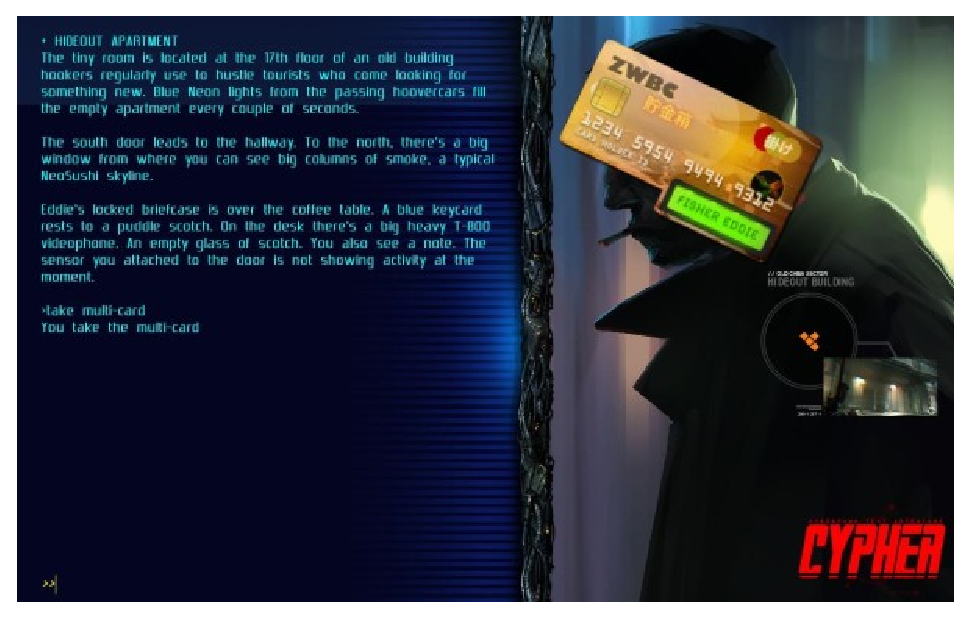
\includegraphics[width=\linewidth]{./media/images/cypher}
  \tiny{\textit{Cypher, an example work of modern interactive fiction (Photo: \href{gameenthusiest.net}{\textsc{gameenthusiest.net}})}}
}
The heart of Interactive Fiction is the medium's hold on people\ldots the way it
washes away your surroundings and transports you to another time and place. I
hope most of all to give the gift of a good story to all.

I give you in this issue a review of some ``old school'' \textsc{if} concepts
tied to modern, practical methods you can use to achieve an experience envisioned by the inspired authors in the past who found themselves
limited by the technology available at the time. My hope is that by using some
or all of the techniques outlined here that you truly immerse your
audience in your story and that they are better for it. 

All in all, I hope you enjoy this magazine. If you like, please feel free to submit your news,
story ideas, questions, and comments. \textit{Discoverer's Digest} seeks to
cover all manner of topics related to \textsc{if}, ranging from parser
experiences to choice\textemdash games, to experiments in the medium (including
General Artificial Intelligence) that we've not yet seen. This is especially true as
\href{https://ifcomp.org/}{\textsc{ifcomp}} is coming up and I'm excited about
that.

To submit you can simply send a personal email to

\href{mailto:cooper@cooper.stevenson.name}{\textsc{cooper@cooper.stevenson.name}}. \\ \\

\noindent Happy Writing! \\ \\

\noindent \href{mailto:cooper@cooper.stevenson.name}{\textsc{D. Cooper Stevenson}}



\chapter*{}
\begin{textblock*}{70.9mm}(0mm,0mm)
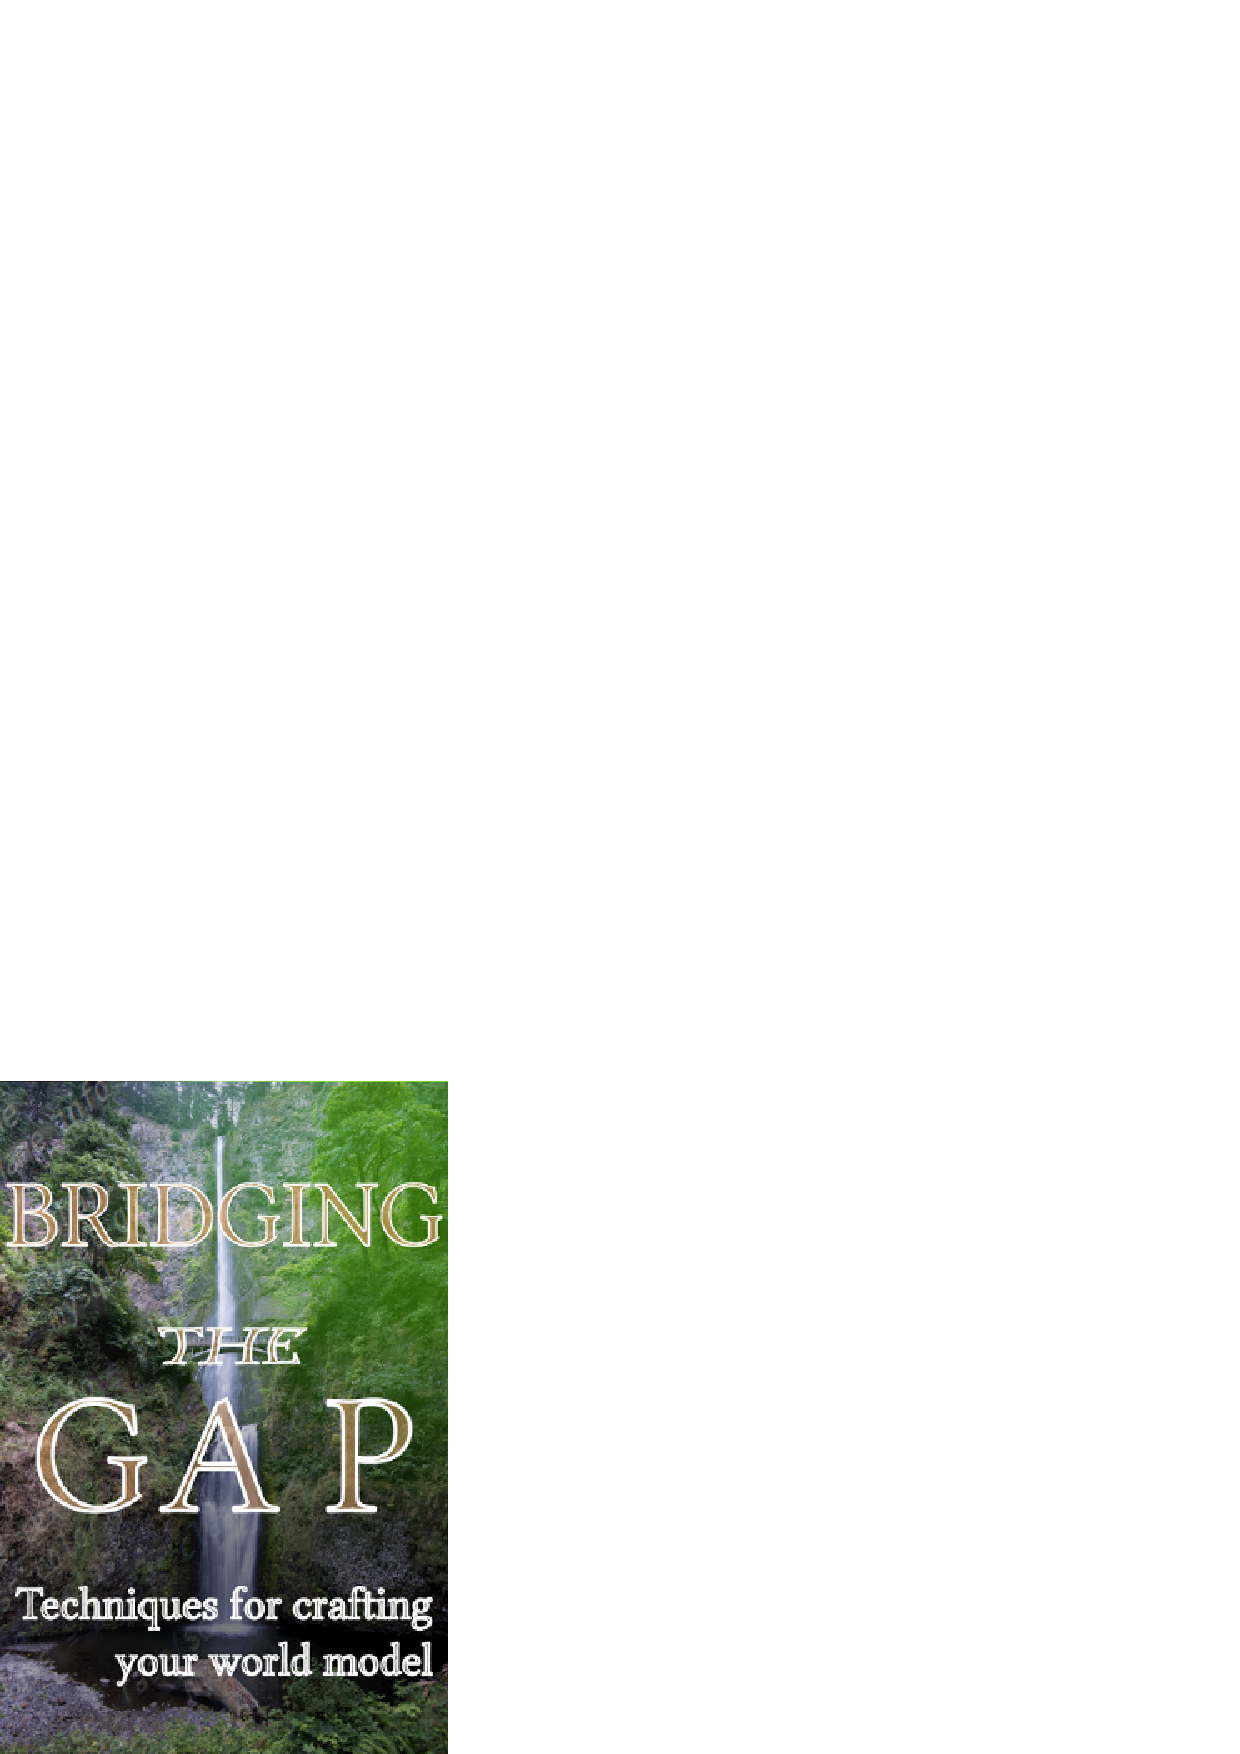
\includegraphics[width=\paperwidth]{./media/images/bridging_the_gap.png}
\end{textblock*}
\chapter{Bridging The Gap \\ \small{Techniques For Crafting Your World Model}}
\begin{figure*}[h]                                                           
 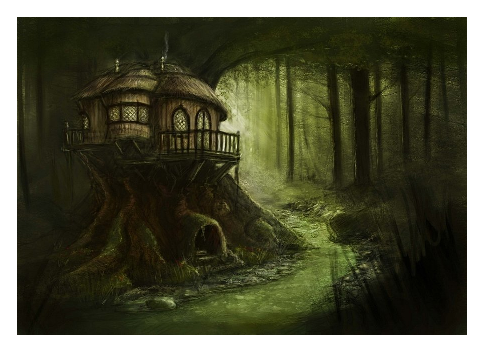
\includegraphics[width=\linewidth]{./media/images/article_one_splash}%
  \small{\textsc{\\ Human perception spans} all our senses and sensibilities.
    Here are a few ways to codify your readers' experience. (Photo: \href{https://www.deviantart.com/tomallica}{\textsc{Tom Walker)}}}
  \label{fig:bridge}%                                                 
\end{figure*}                                                                
\begin{quotation} 
\noindent\color{Sepia}{\scriptsize{\textit{\textbf{“One's
          destination is never a place, but a new way of seeing things.” }}}}\\[2mm]
   \hfill\color{Sepia}{\scriptsize{\textendash Henry Miller}}
\end{quotation} 

\section{museums for the mind}

% ** Story Layer
% *** Room Descriptions
% **** Wikipedia summaries useful here
% **** Multiple Responses for area descriptions
% *** Leave Messages
% *** Arrival Message
% *** Travel Description
% *** Narrator
\lettrine[lines=3]{\color{BrickRed}O}{\enspace ne} of the joys of a good work of Interactive Fiction is the feeling
you get when you interact with the parser on something that you know probably
isn't part of the core for furthering the story but pleasantly discover that
your inquiry works anyway. Even if your interlocutors don't inspect every detail
of their surroundings, just knowing that he is touring a world crafted with care
goes a long way toward immersion.
\marginpar{
  \tiny{\textit{Taking the extra effort and polish to detail your world}}
}
A fleshed out world also, in a practical
sense, implicitely tells the interlocutor that not every object is significant.
This makes the reader have to understand the \textit{solution} the author is
trying to convey as the discovery may be had only through careful thought and
not through, ``Oh, here's a set of keys--these \textit{must} be important.'' A key to a work focused on immersion, I believe, is a world where the author has taken the time to respond intellegently to reasonable inquiries by the player. 

I garner the following factors important to give the reader a sense of immersion:

\begin{itemize}
  \item{Responses for all senses (touch, smell, etc.)}
\item{Differing descriptions based on direction of travel}
\item{Triggered, geography independent narrative}
\item{Multiple responses to the same command}
  \item{Leaving area messages based on conditions}
  \item{Arriving area messages based on conditions}
  \end{itemize}

\marginpar{\vspace{2mm}
  \tiny{\textit{A systematic approach to further your long term story goals}}
}

Fortunately, there are techniques that can help lighten the burden. Developing a systematic approach, at least during the planning phase, can help further your efforts and reduce the feeling that your remaining work is overwhelming.

\subsection{together we stand}
The first and most powerful technique, if possible, is to get help. Make a call
to the Interactive Fiction forums calling for help in areas you may not be
strong. In my case, I am both a good IF architect and writer but my writing is
slow. Someone else may be a good writer but finds ``slaving away'' building the
world model a task that is simply ``beneath'' their artistic talents.
\marginpar{
  \tiny{\textit{Talent wins games, but teamwork and intelligence win championships.}}
}
I, on the other hand, am a facilitator who craves giving artists the ability to
provide the audience with a world model who's prose is constantly fresh,
complete with varying responses based on the direction they're looking, varying
descriptions each time, decorative scenes, and atmosphere. I find the little
things not necessarily adding to the core of the work's message but
\marginpar{\vspace{2mm}
  \tiny{\textit{An ounce of detail is worth a pound of immersion.}}
}
furnishing the world with just a little extra detail immensely
satisfying.  The writer and I are a match made in heaven. The writer is
presented with a beautifully templated world model\textemdash all they need to do is fill in the blanks. I benefit because I can focus on the architecture and each components' relationship to one another.

\section{three layers of interaction}
\marginpar{\vspace{2mm}
  \tiny{\textit{A layered approach.}}
}If we take a work at face value to be focused on the narrative then it makes sense to find a way to weave the narrative in with the world model. This is the difference between a work that the interlocutor \textit{reads} and a work that he \textit{hacks through} looking for clues.


Let's break the work down into three layers, from the lowest to the highest:
\begin{itemize}
  \item{The Reference Layer}
  \item{The World View Layer}
  \item{The Story Layer}
\end{itemize}


\subsection{reference layer}
The reference layer provides the interlocutor with background information about
your world model to be looked up as needed. Several reference models are possible, anything from a notebook carried by the player, a computer terminal in the work, or even spinning rings as in Orson Well's \textit{The Time Machine}. The Reference Layer may even be a physical book or PDF distributed with the work.

Whatever form the factual reference layer takes it's purpose is to enrich the world model and to provide background and orientation to help the reader's success in the work.
\marginpar{\vspace{2mm}
  \tiny{\textit{The reference layer provides a segue to build cognitive world knowledge.}}
}
I don't want to confuse matters, but the reference layer also includes
descriptions of objects and areas after the initial examination/visit. The work
is structured to first give a "flowery" description of an object, for example,
but after that the factual layer takes over and provides a ``clinical'' view of
the scene. You've already weaved the significance of the given object in story form on first review. After this the interlocutor is familiar with this objects relationship in the world space and wishes to concentrate on the practical matter of deciphering the object's meaning in relation to achieving his goals.

\begin{centering}
\includegraphics[width=\textwidth]{./media/images/room_examine.png}
\end{centering}

\subsection{world view layer}
\noindent Moving up from the reference layer is the world view layer. This includes area/object descriptions, the interlocator's sense (sight, smell, touch, etc.) descriptions, and atmospheric spice sprinkled throughout the work.
\marginpar{\vspace{-2.5mm}
  \tiny{\textit{The world view layer grounds the reader in the world model.}}
}
Thousands of pages are written on this topic. The overarching theme is generally this: keep your descriptions sharp, brief and (by design) relevant. Recall that we've broken our work down into three distinct layers. We'll interweave literate prose in this World View Layer in the next layer up, that is, the Story Layer.

\begin{itemize}
  \item{Refined Prose for the initial view, factual view afterward}
  \item{Descriptions dependent on incoming direction}
  \item{Multiple descriptions to reduce tedium}
\end{itemize}
Mechanically, pointing a text summerizer at Wikipedia to boil down complex descriptions of an area to just a few sentances goes a long way to lighten the writer's burden. Place the summarizer's descriptions in your flowchart (outlined below). From here you flesh out the descriptions in your final work. Doing this goes a long way to not feeling like finishing the work is an insurmountable task.

\subsection{story layer}
\label{sec:story_layer}
This literary layer weaves the narrative with the world view layer. It's purpose is to bring narrative to the work--to make your story read like prose. The story layer also can help guide the interlocutor with hints.

\reversemarginpar
\marginpar{\vspace{2mm}
  \tiny{\textit{The narrator fills real\textendash time gaps in the reader's
      thinking, helping him to achieve the next crest of the story.}}
}

I implemented the story layer through three methods in \textsc{tads}. The first is the "initial description" feature, the second by the use of travel messages, and the third a special 'narrator' character who, while not physically existing in the model, injects prose into the work. The narrator is triggered by event state changes.

\normalmarginpar
\marginpar{\vspace{-40mm}
  \includegraphics[width=\linewidth]{./media/images/prop}
  \tiny{\textit{The reader is greeted with ancient proportions in
      The Acropolis (Photo: \href{https://commons.wikimedia.org/w/index.php?curid=156815}{\textsc{joseph kürschner}}}})
}

Here's an example of using refined prose for the initial view:

\begin{quote}
\small{
Propylaea Gateway

Reddish, golden light bathes the tops of the massive walls fortressed against the violet sky.  The contrast of light and shadow sharply mirrors
the angles of the opposing walls relative to the rising sun.  Below the sun's grasp lies softer, luminous blue light making angled pockets of
shadow.  Dew lightly covers the ground and continues up the walls where it glistens as tiny, fractured rainbows above the shadowed relief.  The
air is fresh and slightly chilly with an awakening smell of moist clay.

Beyond the wall's opening to the northeast lie a wide flight of steps rising 40 meters and stretching roughly 25 meters wide.  The steps end to
meet a large six-columned Doric facad at the top.

A scholarly man somewhere in his mid-sixties reads from a scroll nearby.  His calm posture looks to Xantius as he's patiently waited for a
thousand years.  He wears a white robe with a red sash draped around his
shoulders to his mid-section.
} % end small
\end{quote}

\noindent Okay, noting earth shattering here\textendash IF writers have used this
technique for years. You get to exercise your writing chops and, most
importantly, the reader is greeted with engaging prose. Your
descriptions speak directly to the reader. If we've ``gotten out of the way''
and formed a direct conduit to the reader we've done our job.

Let's move from here northeast up the Proplyaea's steps through the archway of
the fortressed wall. Initially, the interlocutor reads thus:

\begin{quote}
  \small{
Propylaea Steps

Moving higher, Xantius's footsteps echo from the steps' sides, where he is now about halfway up.  The Proylaea steps rise impressively before
Xantius, stretching across his entire field of view; roughly 100 men could stand shoulder-to-shoulder spanning the steps' width.  The stairs are
divided into three sections by virtue of their varying grades: finer, longer front-to-back cuts in the center shouldered by shallower, steeper
cuts on either side.  The steps continue upwards to a landing.  A narrower and steeper set of stone steps cut inset to the ridge on Xantius's
right.

\textbf{[The Interlocutor moves further up the steps and then back down.]}

Propylaea Steps

The Proylaea steps continue their descent to the Acropolis outer walls before Xantius, stretching his entire field of view.  The steps run higher
above and behind you to a landing A small flight of steps cut into the steps' border wall lead off to your left (South).

\textbf{[The Interlocutor moves further down the steps and then back up again.]}

Propylaea Steps

Xantius moves up the Propylaea steps, this time on the right side where the grade of the steps are steeper.  ``I wonder why they made the outside
grade of the steps steeper than the inside?  Was it so merchants could make it easier for supplies to be delivered by cart to the Acropolis?'' he
thinks, approaching the stone steps leading in from Xantius's right.  Before him the Propylaea steps rise to the upwards to the West Porch

\textbf{> look}

Propylaea Steps

The Propylaea steps rise at roughly a six per cent grade from the southwest to northeast, running roughly 300 meters from the Propylaea to the
stairs' top to the West Porch.

  }
\end{quote}
  
There's a lot going on here. The interlocutor first gets quality descriptive
prose when first encountering an area. When he returns from the area from a
different direction the description adapts itself to the reader's opposite
vantage point. When combined with varying prose dependent on direction of travel
and the environmental messages I mentioned above you breath life into your
story.
\marginpar{\vspace{2mm}
  \tiny{\textit{Varying responses keeps the world model interesting.}}
}
Also, we've varied the description outlining the reader's travel with, ``\ldots moves
up the Propylaea steps, this time on the right side where the grade of the steps
are steeper.'' These small details go a long way toward immersion and reduces tedium.

Notice the last passage, when the reader enters \textbf{\textit{look}}. We know that he's looking for factual
information about his surroundings. A ``just the facts'' description, indeed, is
exactly what we give him (The Propylaea steps rise at roughly six percent grade\ldots). The \textit{look} command is an indicative command as
it indicates what type of response he's looking for.

\subsubsection{all work and no play}
\label{play}

We can leverage the concept of indicative commands by recognizing when the
interlocutor tries things that are just plain silly.

\marginpar{\vspace{2mm}
  \tiny{\textit{Never taking yourself too seriously.}}
}
For example, when the reader is standing in the Propylaea Gateway from the example above all his senses
are available to him. He can smell the air, smell the wall, etc. None of these
commands are silly, per se, except when he tries to \textbf{\textit{lick the wall}}:

\begin{quote}
  \small{
    Propylaea Gateway
    
    \textbf{> lick wall}
    
Xantius extends his tongue and leans close to the wall.  "This is crazy," Xantius
thought, pausing for a moment to consider how he might appear to perplexed on-lookers.
"C'mon, " he godes himself, "go ahead, go ahead and lick it, I 'double-dog' dare you!"
Moving again closer, Xantius's outstretched tongue contacts the rough wall, making
tacid contact pressing to "full-on" docking.  He imagines himself viewed from the side,
his tongue and the wall's permiations now inversely mirroring each other in perfect
relief.

Xantius's laranyx lets out a half cough as the rest of his pie hole is engaged with
this ridiculous show of machismic servitude.  Xantius textures the invading, finely-
particled nip of marble and limestone on his tonque and, in a twist he hadn't
considered, the outter perimeter of his mouth.  His moist breath sucks some of the
wall's material back into the openings surrounding the axis of his acrid folly.

"Congratulations, Xantius," he thought, "you're a hero."

A little eternity passes before Xantius pulls his geology-coated tongue away from the
wall.  He presently gets right to making several paultry facial expressions as he
tries to dislodge the grit from his mouth\textemdash to end the grinding sound of sand emanating
from inside his skull, broadcasting his displeasure in the process.
} %end small
\end{quote}

\noindent Here we ``break the fourth wall'' giving the reader the idea that we've been
thoughtful designing our world and a break from the challenge intrinsic in the
experience.

\subsection{narration, morgan freeman style}

Here is an example of enhancing the story through a narrator as mentioned on
page \pageref{sec:story_layer}. If the protagonist doesn't bother to say hello
to the scholarly man wearing the sash this will happen (please excuse the
terrible writing):
\begin{quote}
  \small{
    Propylaea Gateway
    
   \textbf{> ne}

Each of Xantius's senses vie for his attention as he pieces together meaning of the
scene before him.  He moves slowly, noticing the "crunch, crunch" of the paultered
ground under his feet turning to a paddled beat on the marble steps.  With his footing
tentatively stepping upward on the Propylaea steps, he raises his gaze upward,
naturally straining his neck higher as he sizes up the ascent's rising to the six-
columned Doric facad marking the entrance of the Acropolis proper.

"What kind of civilization builds a place like this?"  Xantius asks himself, "If such
a place on earth hadn't existed prior to time of the Acropolis's conception, who
envisioned the city...what genius created it?"

Pausing, Xantius breathes in the the dense, moist air breezing in from the nearby
Medditerranian Sea.

Xantius suddenly realizes, "I hadn't gotten that man's name!  I have many questions, to not
sieze the opportunity to speak with him again is to betray it."
    } %end small
\end{quote}

\noindent When Xantius travels after having met the man, Xantius is greated with the
varied travel/description prose as described above plus this bit (again, please
excuse the corny dialog):

\begin{quote}
  \small{
    Propylaea Gateway
    
    \textbf{> ne}
    
   \textbf{[Story travel/description dialog]}

   ``I just met Socrates.  The.  Socrates.  Xantius bolted at the idea. I have so many
questions to ask him!''

\ldots
  }%end small
\end{quote}

\section{tying loose ends}
In the next issue of \textit{Discover's Digest} I'll include more specific
examples and code snippets for applying the layering techniques we discussed above.
% In Chapter \ref{ch:implement} on page \pageref{ch:implement} I'll include structure and code snippets for implementation details.

\chapter*{}
\begin{textblock*}{70.9mm}(0mm,0mm)
\includegraphics[width=\paperwidth]{./media/images/planning_if.png}
\end{textblock*}

\chapter{Sketching Your Reality \\ \small{Tips For Authoring}}
\begin{figure*}[h]                                                           
 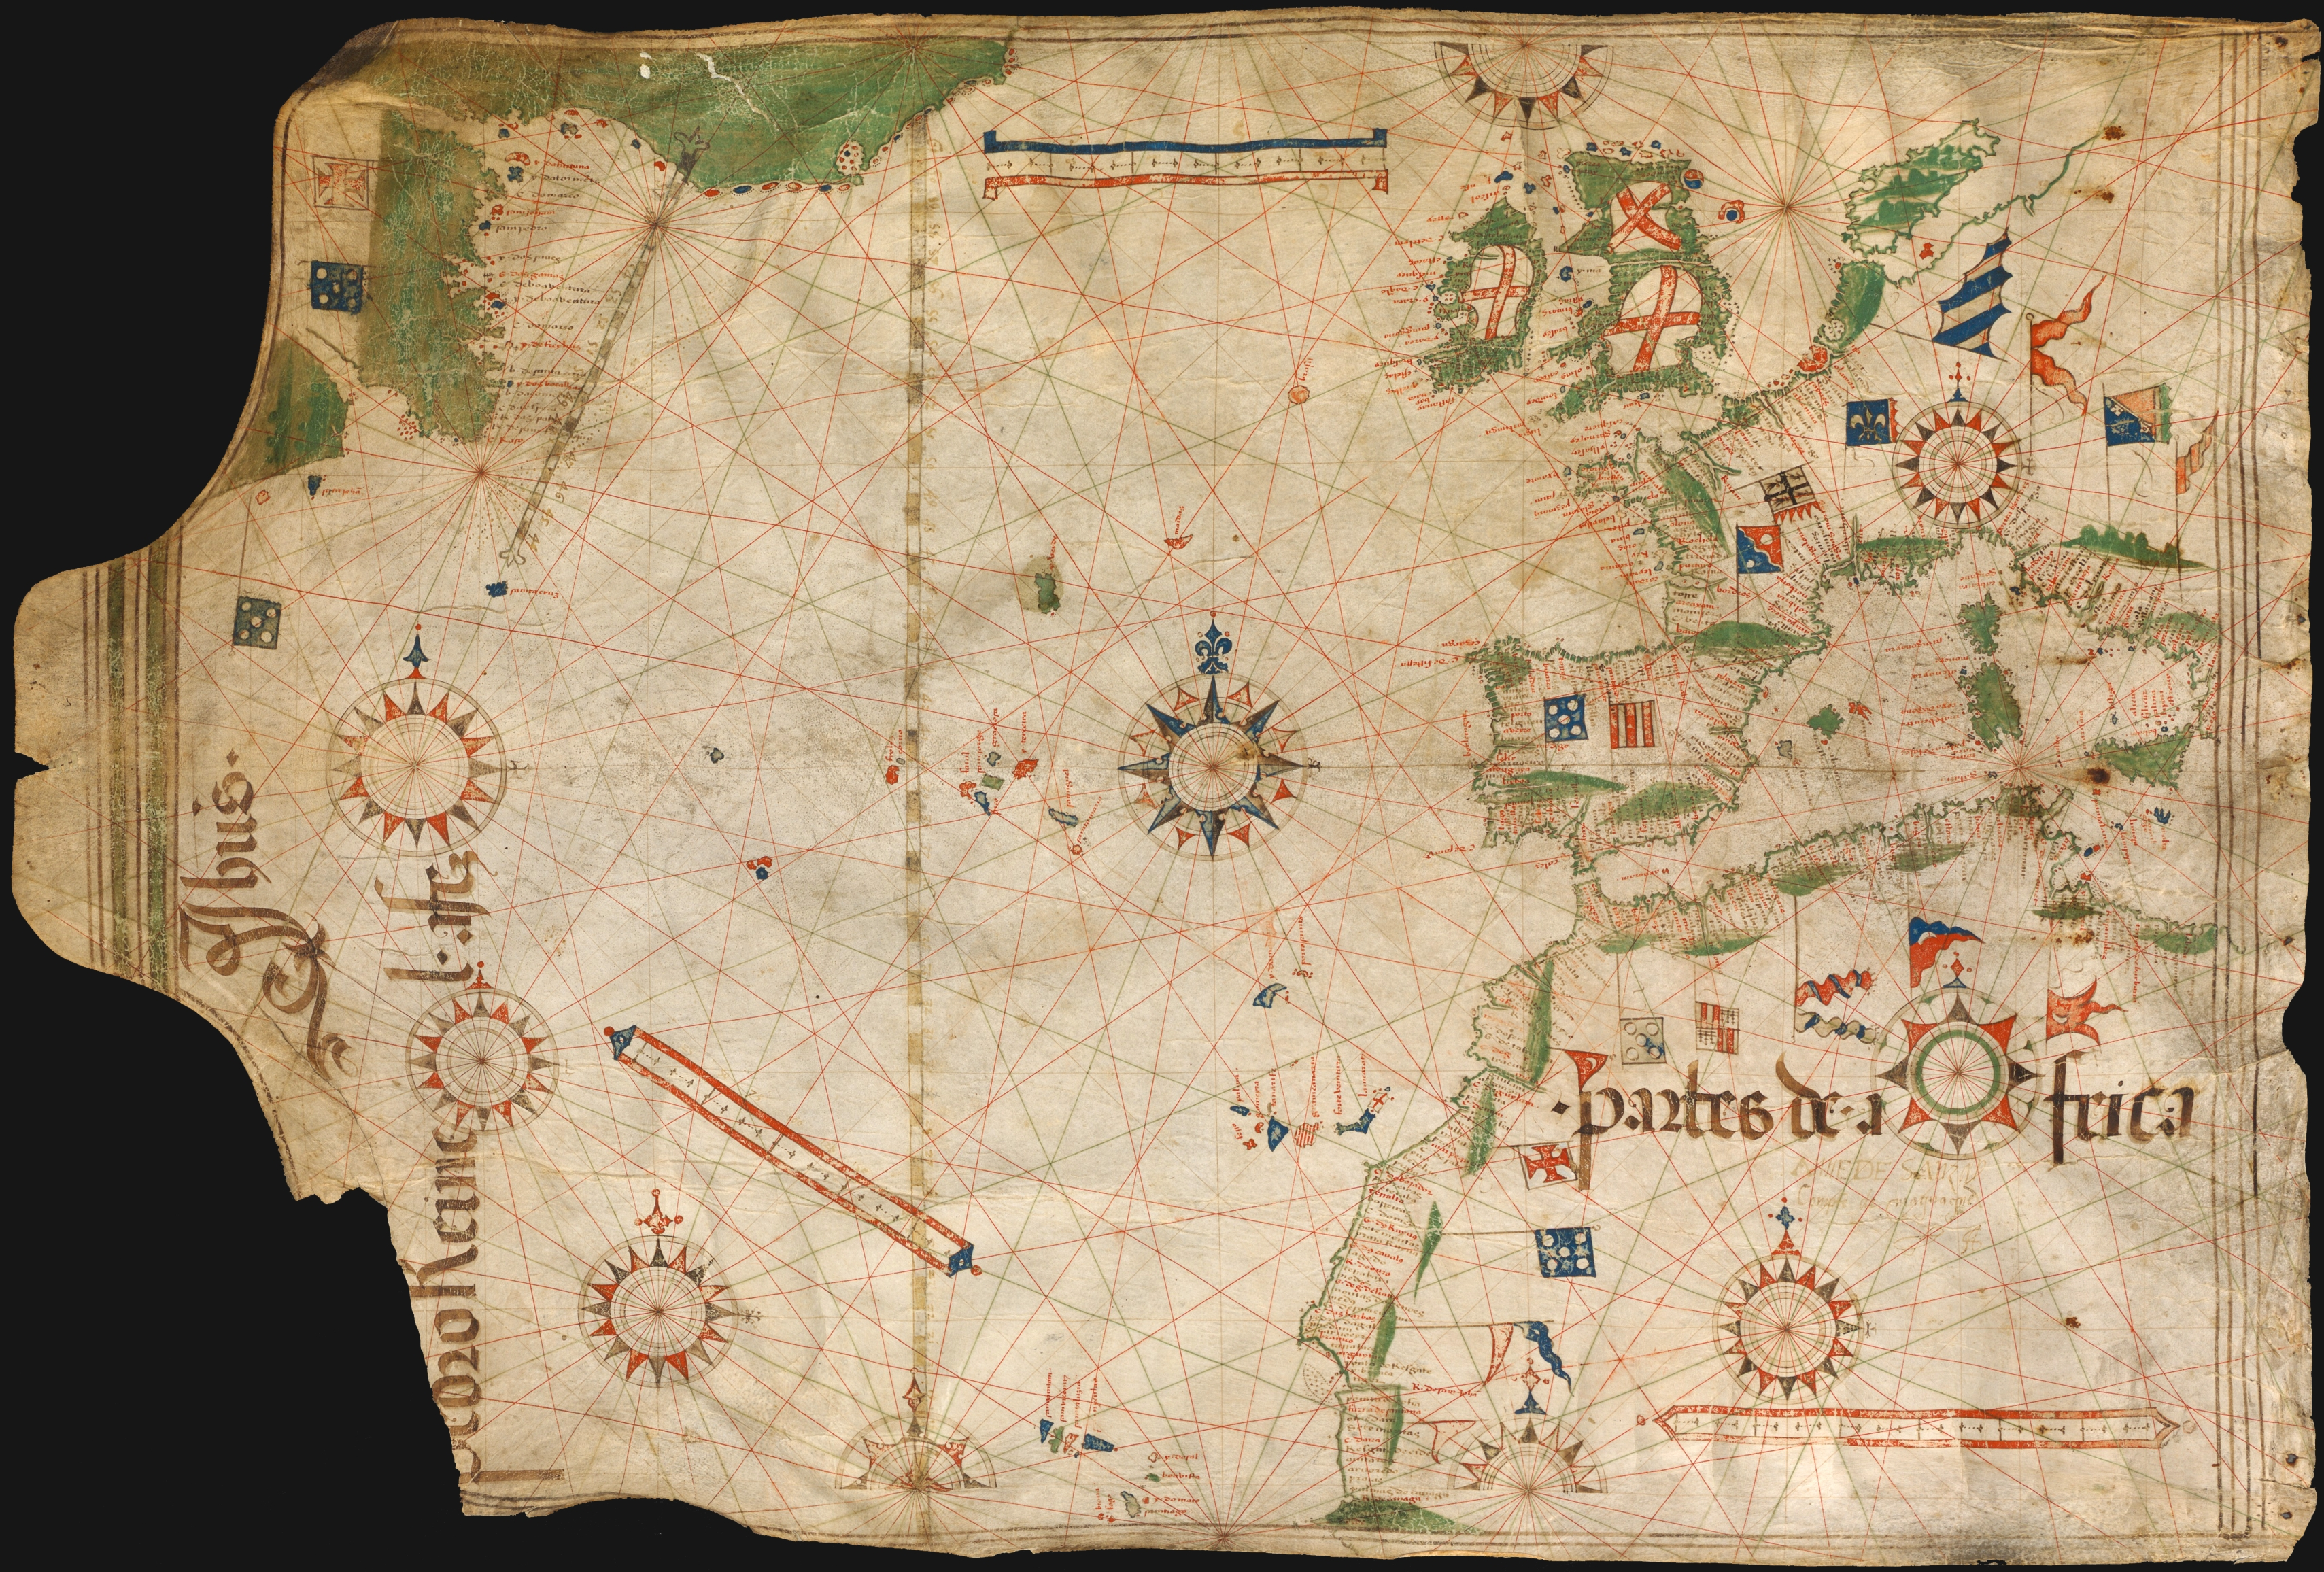
\includegraphics[width=\linewidth]{./media/images/chart}%
  \small{\textsc{\\ Planning your adventure} doesn't have to be a slog\textemdash
    here are some tools to help (Photo:
    \href{https://en.wikipedia.org/wiki/File:Pedro_Reinel_1504.jpg}{\textsc{Bayerische Staatsbibliothek, Munchen).}}}
  \label{fig:planning}%                                                 
\end{figure*}                                                                
\begin{quotation} 
\noindent\color{Sepia}{\scriptsize{\textit{\textbf{“Reality is merely an illusion, albeit a very persistent one..” }}}}\\[2mm]
   \hfill\color{Sepia}{\scriptsize{\textendash Albert Einstein}}
\end{quotation} 

\lettrine[lines=3]{\color{BrickRed}S}{\enspace o} you have an idea for your work of Interactive Fiction. You've mulled the idea
around for some time\textemdash now it's time to start putting your thoughts on
paper (or screen, as it were) but where to start?
\marginpar{\vspace{-2mm}
  \tiny{\textit{Ready, set, go!}}
}

There is no One Way to build a work of IF. Like authorship itself, some writers
like to plan their work ahead of time. Others like to simply spring their writing
spontaneously. Still other authors like to work between a combination of the two.
\marginpar{
  \tiny{\textit{Planning is the key but it's better feeling unconstrained about
      the order of execution}}
}
Where IF differs from traditional authorship is the necessity for at least some
degree of planning. There are many methods for sketching out your work and I
make no constraints for the order by which you choose to build your world model.
You will likely find yourself iterating between the various layers of your work.
There is no need (and I would argue not as effective) to complete one layer
before beginning the next.

Simply by necessity of categorizing the craft of IF I offer the following broad
layers for producing quality work.

\section{physical world layer}
%cover image credit: https://en.wikipedia.org/wiki/File:CMMI_Project_Planning_%E2%80%93_Process-data_model.png
Your overall plot in mind probably lends itself to a setting. In the case of
\textit{The Acropolis} the setting is obvious\textemdash oddly enough, the
Acropolis itself. If you're new to writing IF you will give yourself a leg up on
finishing your product by taking inspiration from a physical location.
\marginnote{
 \includegraphics[width=\linewidth]{./media/images/star_map}%
  \tiny{\textit{\\ There exists virtually no end of maps you can use to inspire your work, including star maps (Photo:
    \href{https://www.classe.cornell.edu/~seb/celestia/pell/images/alliance-union-trade-routes.jpg}{\textsc{celestia
        screen capture).}}}
  \label{fig:starmap}%
  }
}
You also serve yourself as your work will ``feel'' real, similar to the way the venerable \textit{Colossal Caves Adventure} is revered in no small part because it is based on a real cave. The reader finds himself immersed in
his environment because the work \textit{is} crafted from a real location, free from contrivances.

\begin{figure*}[h]                                                           
 \includegraphics[width=\linewidth]{./media/images/acropolis_map}%
  \small{\textsc{\\ Real maps often} provide an effective source of inspiration (Photo:
    \href{https://commons.wikimedia.org/wiki/File:Plan_of_the_Athenian_Acropolis.jpg}{\textsc{A classical dictionary of Greek and Roman biography).}}}
  \label{fig:planning}%
\end{figure*}
A helpful method is to download a map and overlay your IF's map concept over that by

\reversemarginpar
\marginpar{\vspace{8mm}
  \tiny{\textit{Drawing inspiration and templating from real\textendash world
      source material.}}
}
drawing boxes over each location with connectors in\textendash between.
\textit{Inkscape}'s connector tool is effective for this as it gives you freedom
to place your locations wherever you like while taking care of the connector
details.


If you prefer a templated approach\textemdash one that will build a world model
for you after you've finished your map\textemdash
\href{http://ggarra13.github.io/ifmapper/en/}{\textsc{if mapper}} and
\href{https://trizbort.genstein.net/#overview}{\textsc{trizbort}} are two utilities to do
this. If you prefer a programmatic approach,
\href{https://ifm.readthedocs.io/en/latest/}{\textsc{ifm}} lets you create a map from a
text file. \href{https://github.com/dustinlacewell/t3sketch}{\textsc{t3sketch}} offers a
complete templating system for \textsc{tads3} (including build tools) to lay
down your world model (Hint: use the included xml file in the respository
\texttt{\tiny{t3sketch/example/living\_quarters.xml}} to get started).

\subsection{composing the scene}
You may find
\reversemarginpar
\marginnote{\tiny{\textit{Visiting a location and writing everything
      about it inspires}}}
 yourself in a place where you've mapped your story (at least
partially) and find yourself with a myriad of empty location boxes needing a
description. One method I 'stole' from the excellent
\href{https://www.amazon.com/Travel-Writing-World-Sell-Story/dp/1582973814}{travel
writing: see the world. sell the story} book is to physically visit a location
with your notebook and simply, ``write like hell.'' Capture everything you're
experiencing in this location as scribbles\textemdash just get it all down. 
\normalmarginpar
\marginnote{
  \includegraphics[width=\linewidth]{./media/images/celestia}
  \tiny{\textit{Celestia's ``free range'' space exploration system
      means you can accurately plot a universe for your work of Science Fiction (Photo:
      {\href{https://www.cyberciti.biz/tips/celestia-astronomy-linux-program.html}{
          Vivek Gite, nixCraft}})}}
  }
Record the sights, both local and distant, the smells, the sounds, etc. Your
location needn't necessarily be one similar to the locations in your work of IF
as you're almost certain to draw inspiration from your ``fast and furious''
writing on location.
\reversemarginpar
\marginnote{\tiny{\textit{Text summarizers are helpful for quickly drafting locations}}}
Another good way to fill in the boxes is to summarize works of text found on the
Internet that resemble your location with a natural language summerizing tool
like \href{https://github.com/miso-belica/sumy}{\textsc{sumy}}. Simply point
to your location description's \textsc{url} and let it generate a few
sentences about your location. Here's an example of the summarizer pointed to a
description of the Parthenon:

\begin{quote}
  \small{
\noindent \textbf{\$ sumy lex-rank --length=10 --url https://www.ancient.eu/parthenon/}

\noindent The magnificent temple on the Acropolis of Athens, known as the Parthenon, was built between 447 and 432 BCE in the Age of Pericles, and it was dedicated to the city ’s patron deity Athena.

From the 4th century BCE the whole building acquired the name Parthenon. The Parthenon would become the largest Doric Greek temple, although it was innovative in that it mixed the two architectural styles of Doric and the newer Ionic.

It was entered through large wooden doors embellished with decorations in bronze, ivory, and gold. The temple was unprecedented in both the quantity and quality of architectural sculpture used to decorate it.

The pediments of the temple measured 28.55 m in length with a maximum height of 3.45 m at their centre.

Many of the metopes on the other sides of the building were deliberately damaged and figures in the central part of the east pediment were removed.
} %end small
\end{quote}
\noindent Not bad. You've now a foothold by which to base your descriptions;
``slice and dice'' your summary to suit.

\section{a picture worth a thousand words}
Now we've mapped a framework for our world using a map tool, and used a summarizer
for each locations' description let's suppose we'd like to add images for some or all
of our locations.
  \marginpar{
    \includegraphics[width=\linewidth]{media/images/artistic_scenery}%
  \tiny{\textsc{\\ An artistic means} of capturing your readers' attention by the tasteful use of color on black\textendash and\textendash white (Photo: \href{https://pixabay.com/en/artistic-scenery-black-and-white-60871/}{\textsc{Pixabay: ``Steppinstars'').}}}
} %end marginpar
\begin{figure*}[h]                                                           
  \includegraphics[width=\textwidth]{./media/images/exoplanet}
  \small{\textsc{Imagine your interlocutor as} the first to discover
      organic molecules with the help of freely available NASA images (Photo:
      \href{https://images.nasa.gov/details-PIA21470.html}{\textsc{nasa/jpl-caltech}})}
  \label{fig:nasa}
\end{figure*}

Obviously, pointing a search engine looking for appropriately licensed images
will do some of the job, and there are plenty of free resources for you to
include in your work. \href{https://pixabay.com/en/photos/}{\textsc{pixabay}},
\href{https://en.wikipedia.org/wiki/Wikipedia:Images}{\textsc{wikimedia}}, and
\href{https://pikwizard.com/}{\textsc{pikiwizard}} are all available to name a
few. Eric Matyas, by the way, offers a wide range of
\href{https://soundimage.org/}{\textsc{images and sound e{ff}ects}} available for
\textsc{if} authors; you need only provide the appropriate attribution for his work.

\subsection{blender}
\marginnote{
  \includegraphics[width=\linewidth]{./media/images/acropolis_model}
  \tiny{\textsc{A 3D Model} \textit{of the Acropolis is free for download and use (Photo: {\href{https://www.blendernation.com/2012/11/30/model-download-acropolis-of-athens-165ad/}{Sebastian Kiersz}})}}
  }
\noindent Having a free, full\textendash fledged 3D modeler is tough to beat for giving
your readers a graphical way to orient themselves in your world model.
Complete agency extends as far as your imagination. It's not hard to imagine a
super\textendash imposed compass rose on the floor of each location to further
ease the interlocutor's navigation through your world. In the case of \textit{Acropolis} a \href{https://www.blendernation.com/2012/11/30/model-download-acropolis-of-athens-165ad/}{\textsc{ready\textendash made model exists}}.
\subsection{flight simulator}
You can map out entire outdoor spaces using
\marginnote{
  \includegraphics[width=\linewidth]{./media/images/fg_map}
  \tiny{\textit{FlightGear's map modelling software makes making good\textendash
      looking maps easy (Photo:
      \href{http://geoffmclane.com/fg/atlas-07.htm}{\textsc{geoff mclane}}})}
}
\href{http://home.flightgear.org/}{\textsc{flightgear}}'s mapping and view
options. Flightgear is quality open source flight simulator that is available
for free download. You can use Flightgear to map out accurate \textsc{gis}
experiences or as an inspiration to an environment of your creation.
\begin{figure*}[h]                                                           
 \includegraphics[width=\linewidth]{./media/images/fg_scenery}%
  \small{\textsc{\\ FlightGear offers detailed }\,\& stunning views of natural
    terrain (Photo:
    \href{http://www.flightgear.org/wp-content/uploads/2014/09/dds-regional-ALS.jpg}{\textsc{Flightgear
        project).}}}
  \label{fig:fg_scenery}%                                                 
\end{figure*}                                                                
First, use the \href{https://www.maps.ie/coordinates.html}{\textsc{a map tool supporting latitude/longitude coordinates}} to plot the points you want to
describe. Then use FlightGear's ``\textsc{ufo} mode'' to place your location precisely where you want
it. You can use either a screenshot tool or FlightGear's built\textendash in
tool to capture the scene. If you're really ambitious you can capture a scene
for each compass direction should the interlocutor type a look directive with a
specific direction like \texttt{\small{>\,look east}}.

\marginnote{
  \includegraphics[width=\linewidth]{./media/images/fg_sat_map}
  \tiny{\textit{FlightGear's map server is fast and provides detail down to the
      individual tree level (Photo:
      {\href{http://mpmap02.flightgear.org/}{flightgear map server}})}}
  }
A mapping tool based on FlightGear's data may be had with
\href{http://wiki.flightgear.org/Atlas}{\textsc{atlas}}. You define the area
and features that you want to map and Atlas provides a nice shaded relief map. 

Other sources for map inspiration include \textsc{qgis} geographical information
system software and \href{http://mpmap02.flightgear.org/}{\textsc{flightgear's map server}}. Both these applications
offer stunningly sharp detail.
\subsection{space simulators}
\marginnote{
  \includegraphics[width=\linewidth]{./media/images/stellarium}
  \tiny{\textsc{Stellarium's views offer} \textit{``world-class'' experiences
      (Photo:
      {\href{https://www.star-watcher.ch/equipment/stellarium-app/}{Karol
          Novotny, star\textemdash watcher}})}}
  }
\noindent Space simulators like \href{https://stellarium.org/}{\textsc{stellarium}} and
\href{https://celestia.space/}{\textsc{celestia}} come as ready\textendash made sources
for star maps and scenery. Both offer the ability to locate yourself in any
number of reference points from which to base your story. Imagine a Science
Fiction story who's view out the ship's portal is an accurate depiction of the
location's celestial bodies!

\section{plotting the story layers}
Works of Interactive Fiction that do not (or at least minimally) commit
\href{http://pdf.textfiles.com/books/iftheorybook.pdf}{\textsc{crimes against mimesis}}
require careful planning. When the reader is rewarded having achieved the next
phase of the story to a beautiful scene including, ``golden, sun\textendash
drenched waves splashing against the towering rock formations,'' the last thing
we want our locutor to experience is this:
\begin{quote}
  Gold Beach
  
  \ldots golden, sun\textendash
  drenched waves splash against the towering rock formations in relief.''

  \textbf{> look at rocks}

  You see no rocks here.
\end{quote}

\noindent Plotting isn't limited to your physical world layer; you can use it to map your plot and narrative layers too.

\begin{figure*}[h]
 \includegraphics[width=\linewidth]{./media/images/story_board.pdf}%
  \small{\textsc{\\ Creating a story board} goes a long way toward completion
    and enhancing coherence (Photo:
    \href{http://portfolio.cooper.stevenson.name}{\textsc{Cooper Stevenson).}}}
  \label{fig:storyboard}%                                                 
\end{figure*}
For example, in \textsc{\vref{fig:storyboard}} I lay out the the conversation in Plato's
\href{https://www.gutenberg.org/files/1497/1497-h/1497-h.htm}{\textsc{the
    republic}}. Each character is listed horizontally across the top of the plot. Each topic they discuss, in order, is listed vertically along the
left\textendash side. From here we can create \small{\texttt{ask/tell}} directives for
the compiler.


% to generate diagram
% $ dot -Tsvg conv_short.dot -o conv_short.svg
% then convert to PDF
%This didn't scale well but did manage to get in doc:
% $ dot2tex --figonly --graphstyle "scale=0.5" ./conv_short.dot > /home/cstevens/doc/if/dot.tex
\begin{figure*}[h]
 \includegraphics[width=\linewidth]{./media/images/conv_short.pdf}%
  \small{\textsc{\\ Mapping the story}, bit by bit, from source material. This
    simplified view depicts the plotting process; source
    page numbers references are helpful for
    later fleshing out your story. (Photo: \href{http://portfolio.cooper.stevenson.name}{\textsc{Cooper Stevenson}).}}
\end{figure*}

In the next edition of \textit{Discoverer's Digest} I will include the code
snippets for producing the examples of world/plot/narrative plotting I cited
above.



\chapter*{}
\begin{textblock*}{70.9mm}(0mm,0mm)
\includegraphics[width=\paperwidth]{./media/images/epilogue}
\end{textblock*}

\chapter{Epilogue\\ \small{Where We Go From Here}}
\label{ch:epilogue}
\begin{figure*}[h]                                                           
 \includegraphics[width=\linewidth]{./media/images/engaged}%
  \small{\textsc{\\ Imagine your readers' feeling} knowing they tackled mind and matter to complete the Quest (Photo:
    \href{http:portfolio.cooper.stevenson.name}{\textsc{D. Cooper Stevenson).}}}
  \label{fig:engaged}%                                                 
\end{figure*}                                                                
\begin{quotation} 
\noindent\color{Sepia}{\scriptsize{\textit{\textbf{“Ease of navigation is important in both physical and virtual space.” }}}}\\[2mm]
   \hfill\color{Sepia}{\scriptsize{\textendash John Quelch}}
\end{quotation} 

\section{updates and expansion}
This edition of \textit{Discoverer's Digest} is necessarily a rolling release
edition of the magazine. As Voltaire quotes the Itallian proverb, ``Don’t let
the perfect be the enemy of the good.'' In the next week or so I will update
these articles with the specific code samples necessary to create the plots,
etc. I described in the article. I feel this especially important as
\href{http://ifcomp.org}{\textsc{ifcomp}} is hot underway; should I give just
one author a spark of inspiration to improve his entry I will have considered
this work a sucess.

\subsection{upcoming issue}
In the next issue of \textit{Discoverer's Digest} I tackle in concrete terms
extended areas of \textsc{if} that are sometimes discussed but not, at least as
far as I am aware, fully implemented.

First up brings the power of \textsc{tads} to hook the ``real world'' into your
work of \textsc{if}. Specifically I show an example and code for using
\textsc{gps} in your next adventure. For now I leave you with
\href{http://portfolio.cooper.stevenson.name/tarlatt/tarlatt_slough_trail_feature_demo.mp4}{\textsc{this
    partial walkthrough}} exploring a trail along Willapa Bay in Long Beach, WA.

Also, I'll build on the plotting I described in this issue to explore using
Natural Language Processing to make ``filling in the blanks'' of your work
faster, fuller, and comprehensive.

\subsection{``adieu'' \& additions}
Your sumissions of news, musings, or reviews/announcements of new works are
always welcome. Simply \href{mailto:cooper@cooper.stevenson.name}{\textsc{send
    me a personal email}} to submit.

Until next time (and as always), I wish you the best in your enjoyment of the
medium! \\ \\

\noindent Fair Winds, \\ \\

\noindent \href{mailto:cooper@cooper.stevenson.name}{\textsc{D. Cooper Stevenson}} 



%\chapter*{}
%\begin{textblock*}{70.9mm}(0mm,0mm)
%\includegraphics[width=\paperwidth]{./media/images/engaged}
%\end{textblock*}
%\chapter{IF In The Real World \\ \small{GPS-Enabled Adventures for Exploration}}
%\label{chap:real_world}
%\begin{figure*}[h]                                                           
 \includegraphics[width=\linewidth]{./media/images/engaged}%
  \small{\textsc{\\ Imagine your readers' feeling} knowing they tackled mind and matter to complete the Quest (Photo:
    \href{http:portfolio.cooper.stevenson.name}{\textsc{D. Cooper Stevenson).}}}
  \label{fig:engaged}%                                                 
\end{figure*}                                                                
\begin{quotation} 
\noindent\color{Sepia}{\scriptsize{\textit{\textbf{“Ease of navigation is important in both physical and virtual space.” }}}}\\[2mm]
   \hfill\color{Sepia}{\scriptsize{\textendash John Quelch}}
\end{quotation} 

\section{updates and expansion}
This edition of \textit{Discoverer's Digest} is necessarily a rolling release
edition of the magazine. As Voltaire quotes the Itallian proverb, ``Don’t let
the perfect be the enemy of the good.'' In the next week or so I will update
these articles with the specific code samples necessary to create the plots,
etc. I described in the article. I feel this especially important as
\href{http://ifcomp.org}{\textsc{ifcomp}} is hot underway; should I give just
one author a spark of inspiration to improve his entry I will have considered
this work a sucess.

\subsection{upcoming issue}
In the next issue of \textit{Discoverer's Digest} I tackle in concrete terms
extended areas of \textsc{if} that are sometimes discussed but not, at least as
far as I am aware, fully implemented.

First up brings the power of \textsc{tads} to hook the ``real world'' into your
work of \textsc{if}. Specifically I show an example and code for using
\textsc{gps} in your next adventure. For now I leave you with
\href{http://portfolio.cooper.stevenson.name/tarlatt/tarlatt_slough_trail_feature_demo.mp4}{\textsc{this
    partial walkthrough}} exploring a trail along Willapa Bay in Long Beach, WA.

Also, I'll build on the plotting I described in this issue to explore using
Natural Language Processing to make ``filling in the blanks'' of your work
faster, fuller, and comprehensive.

\subsection{``adieu'' \& additions}
Your sumissions of news, musings, or reviews/announcements of new works are
always welcome. Simply \href{mailto:cooper@cooper.stevenson.name}{\textsc{send
    me a personal email}} to submit.

Until next time (and as always), I wish you the best in your enjoyment of the
medium! \\ \\

\noindent Fair Winds, \\ \\

\noindent \href{mailto:cooper@cooper.stevenson.name}{\textsc{D. Cooper Stevenson}} 




% Going to Canon beach to take pictures
% - Getting back after dark

% bored waiting me to take picture of valley farm


\end{document}
